
In this section, we present the general design of a self-driving system and
under what conditions it may fail, e.g., the computer system cannot 
understand the semantic meanings of road/traffic conditions. 
Augmenting vehicles with remote-control operations is not a new 
concept. For example, \cite{kang2018rc} has discussed some of the key challenges
in designing such a system. The focus of our paper, instead, is in addressing
many of these challenges and in designing a more end-to-end demonstration
of the proposed capability.



\begin{figure*}[ht]
\centering
  \begin{subfigure}[t]{0.33\textwidth}
    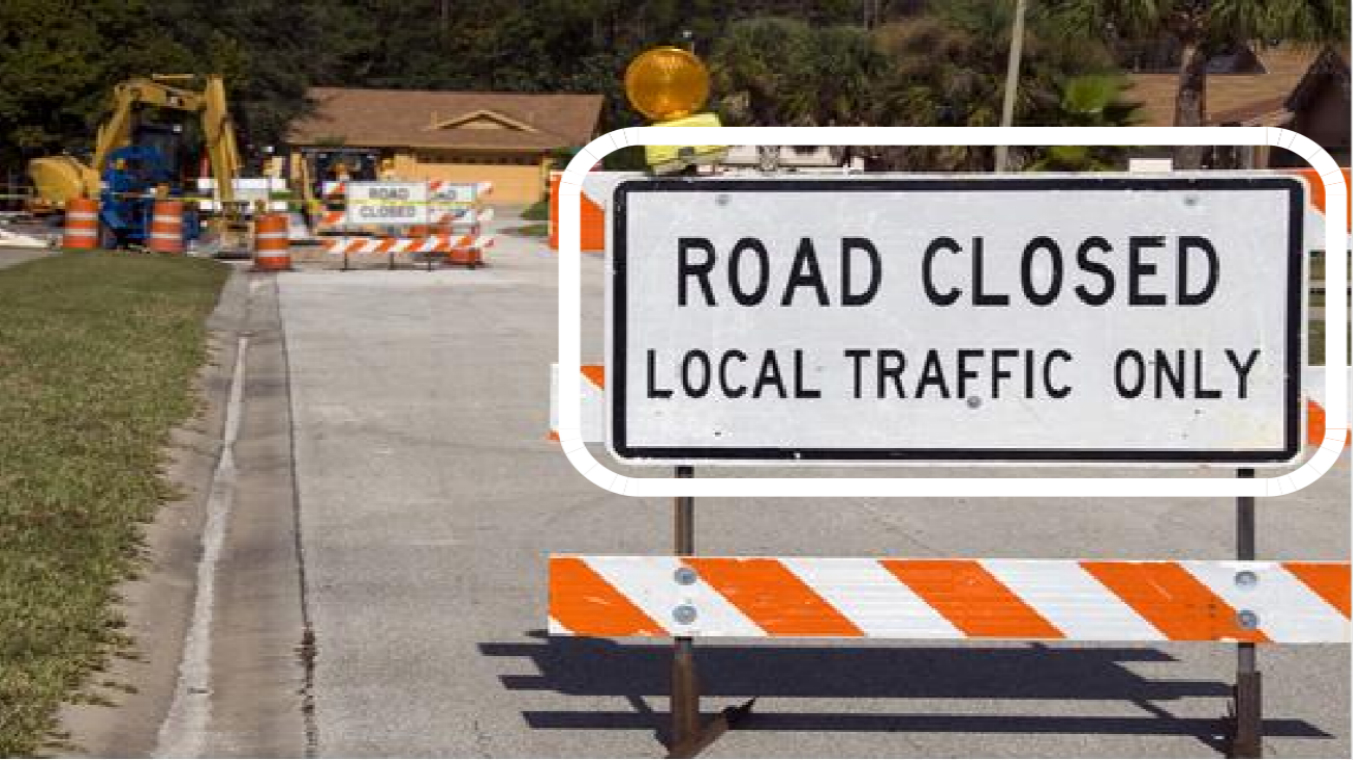
\includegraphics[width=\linewidth]{Figs/RTDrive/motivation/local_traffic.jpeg}
    \vspace{-0.2cm}
    \caption{Instruction with complex semantics.}
    \label{motivation:local_traffic}
  \end{subfigure}%
 \begin{subfigure}[t]{0.33\textwidth}
    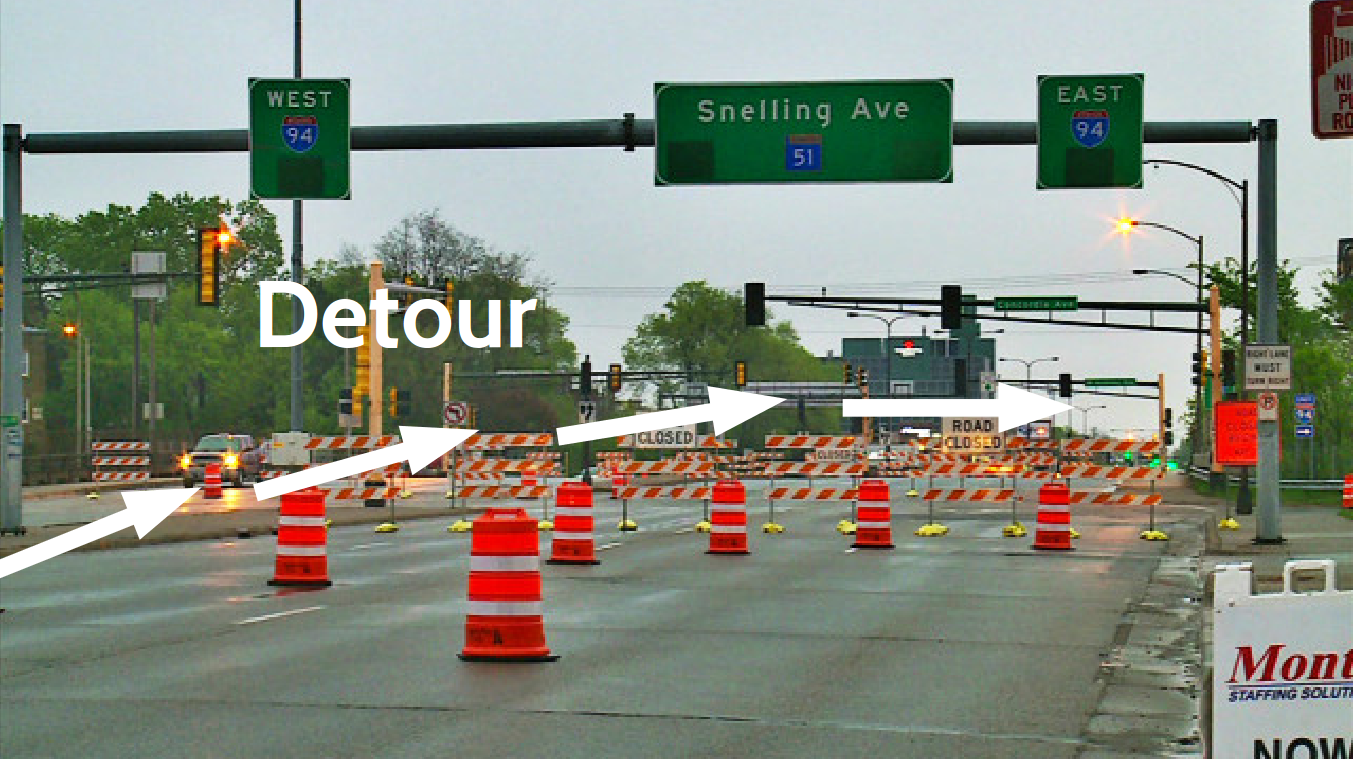
\includegraphics[width=\linewidth]{Figs/RTDrive/motivation/detour.jpg}
    \vspace{-0.2cm}
    \caption{Confusing detour arranged by barrels.}
    \label{motivation:detour}
  \end{subfigure}%
  \begin{subfigure}[t]{0.33\textwidth}
    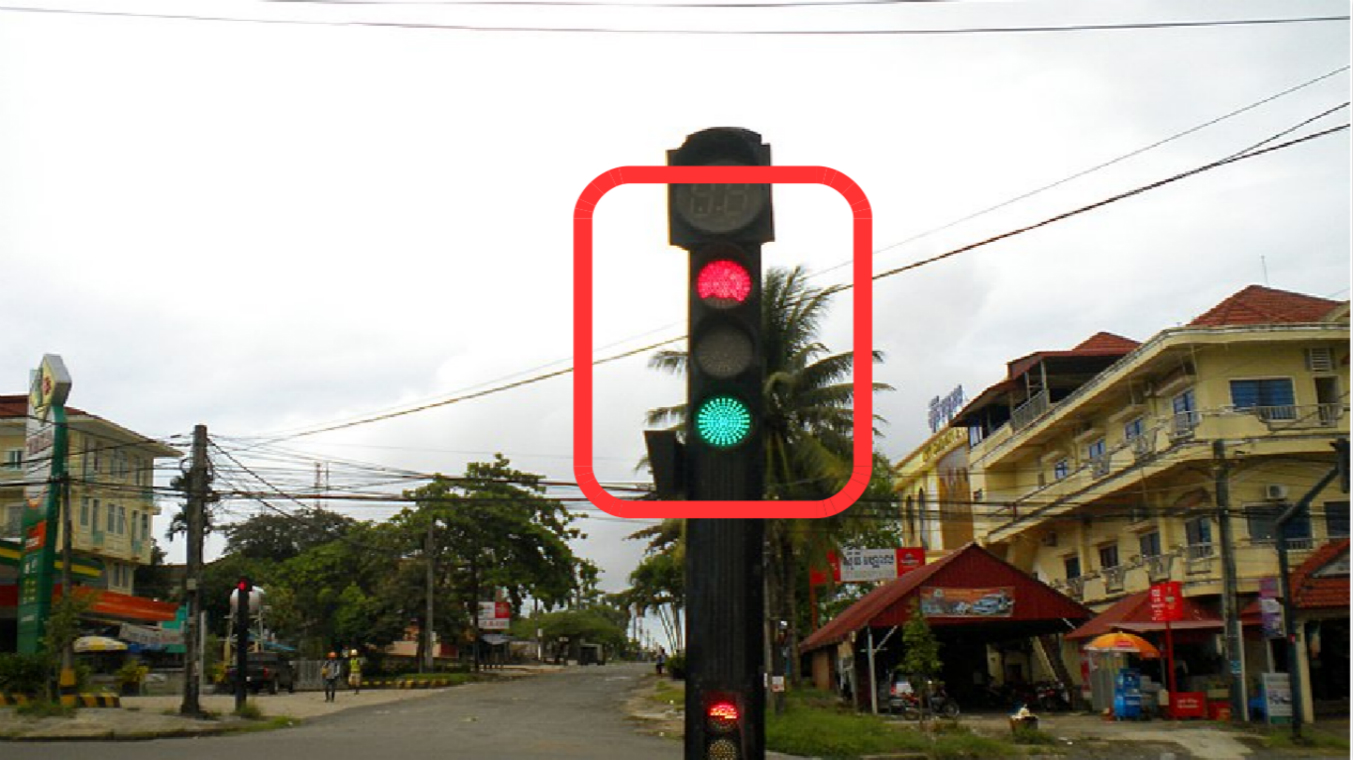
\includegraphics[width=\linewidth]{Figs/RTDrive/motivation/malfunctioning_traffic_light.jpg}
    \vspace{-0.2cm}
    \caption{Malfunctioning traffic lights.}
    \label{motivation:malfunction}
  \end{subfigure}%
  \vspace{-0.3cm}
  \caption{Self-driving system may occasionally fail under diverse real world conditions.}
  \label{motivation}
  \vspace{0.0cm}
\centering
\end{figure*}


\subsection{Self-Driving System Overview}


A self-driving system consists of several modules that are responsible for
different functionalities, i.e.,  
perception, localization, planning and control \cite{pendleton2017perception}. 
Perception refers to the ability to collect information and extract
relevant knowledge from the environment, 
such as detecting obstacles, identifying lane markers,
and categorizing these data by their semantic meanings. 
Localization refers to the ability to determine the 
vehicle's position with respect to the environment. 
Planning refers to the process of making purposeful decisions 
in order to navigate the vehicle 
while avoiding obstacles and optimizing over designed heuristics.
Finally, a control module is used to execute the planned actions.
Similar to human drivers, self-driving vehicle follows predefined traffic rules, 
such as drive within lane, do not cross double yellow line (except left turns),
stop at the red traffic light (except right turns in certain cases) etc. 
The perception module is used to understand the environment 
and traffic rules. 
If the perception module fails to do so, the vehicle may try to park
safely or operate with undefined actions \cite{waymo}.  

\subsection{Self-Driving System Failure Analysis}
\label{sec_failure}

We present several challenge conditions that a self-driving system
may fail if such conditions are not considered at system
design time. 


\textbf{Road sign or instruction with complex semantics}. 
The road sign or instruction can be too complex to be 
understood by self-driving system. 
One such example is illustrated in Fig. \ref{motivation:local_traffic}, 
where the road is closed and only local traffic is allowed. 
The self-driving system could fail to understand 
the semantics of ``local traffic'' or
fail to understand if it belongs to ``local traffic''.
Other complex semantics of instructions include
specific dates, specific type of vehicles 
and street names. 
If the self-driving system cannot understand road sign 
or instruction, it needs further human input. 


\textbf{Confusing and complex detour}.
Confusing detour due to misplaced cones or complex instructions 
may cause self-driving system failure. 
As shown in Fig. \ref{motivation:detour}, an experienced driver
can follow the barrels and drive out of the road boundaries
to pass this area, while a self-driving system may 
fail to identify a detour. 
Since there is no specific rules to place
traffic barrels, it is hard to find a general logic to 
learn where the detour is. 
There are also detour instructions that specify the street
name, exit number, special event instructions, 
that are too complex to be handled
by self-driving systems.
In such conditions, human knowledge and inputs are required. 

\textbf{Confusing or malfunctioning traffic lights/signs}.
Malfunctioning traffic light may cause self-driving
system failure as well. 
One example is shown in Fig. \ref{motivation:malfunction}, 
the traffic light turns to both red and green, 
and the self-driving system may fail to understand 
the traffic light is malfunctioning and act
with undefined behaviors.
Accidents may happen if all the traffic lights turn green at
an intersection.  
There are also confusing traffic light (e.g., yellow left turn light etc.)
and road signs (e.g., no right turn on red etc.) that
could need human inputs
\footnote{\url{https://www.youtube.com/watch?v=femUe6bds0U}}. 



\textbf{Perception failure at night and more}
Visibility and weather conditions are challenging for self-driving 
systems as well, 
i.e., low visibility due to fog \footnote{\url{https://www.youtube.com/watch?v=uYav3_7miIc}},
lane markers are covered by snow
\footnote{\url{https://www.youtube.com/watch?v=fc0yYJ8-Dyo}}.
There are also other conditions that are so complex
that a computer system may fail to handle, such as 
LIDAR or camera failures \cite{waymo}.


\subsection{Remote View and Control}


\begin{figure}[t]
\centering
\vspace{-0.2cm}
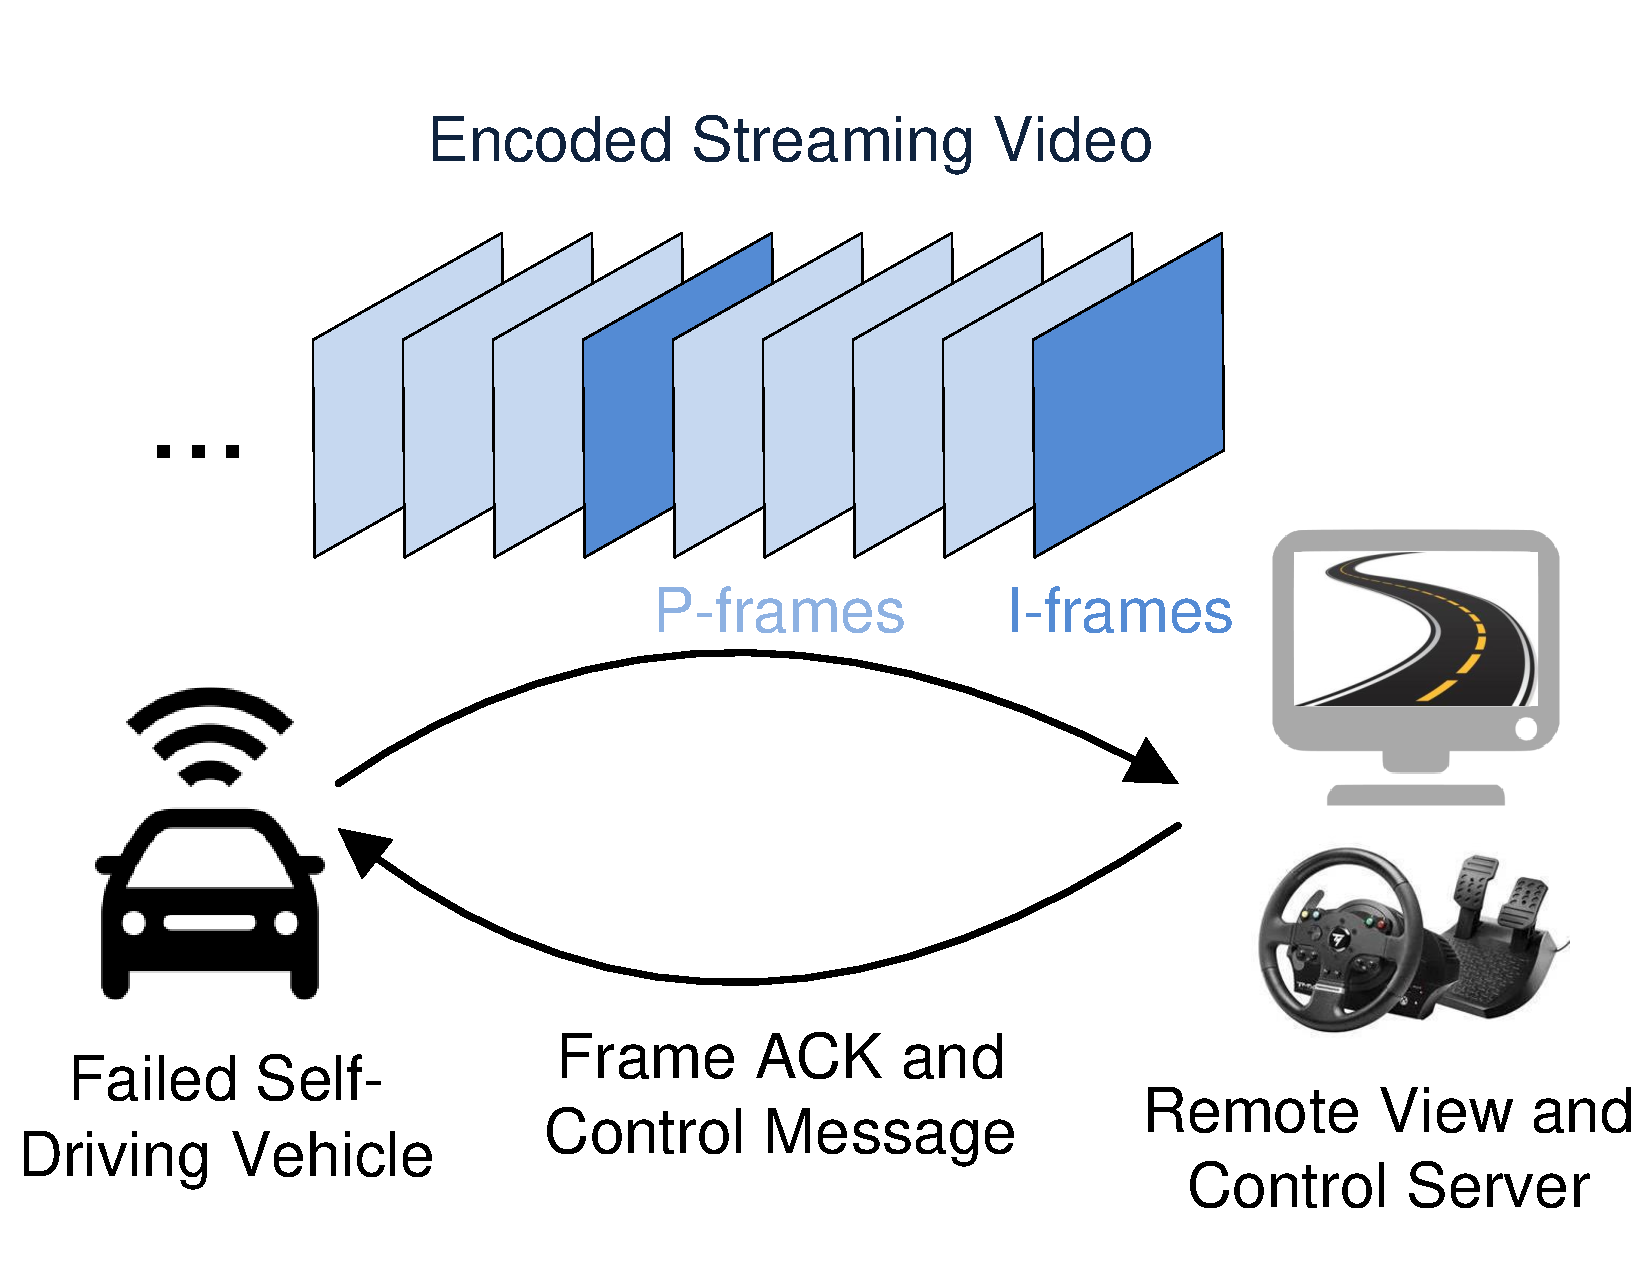
\includegraphics[width=2.6in,angle=0]{Figs/RTDrive/illustration.pdf}
\vspace{-0.4cm}
\caption{Remote view and control server to augment self-driving systems
(only when the self-driving system fails).}
\vspace{-0.4cm}
\label{illustration}
\centering
\end{figure}

With the possibility of failure in the complex road or traffic
conditions, remote view and control systems can act as a safe backup
of self-driving systems, 
i.e., the view and control can be transferred to the remote
operator upon these occasional failures describe in section \ref{sec_failure}. 
It also releases the human drivers behind the wheel who take over the 
control after system failures \cite{waymo}. 
A high level architecture is illustrated in Fig. \ref{illustration}.  
Upon system failure, the view of self-driving vehicle
is sending to the remote server, 
and the operator can view and control the vehicle in real time. 
Suppose a road lane is closed due to road work, 
a self-driving system can simply detect
that the current lane is blocked,
while it may fail to understand the semantic meanings
of the road signs. 
The remote human operator can take over the control and 
return the control to the self-driving system once the vehicle pass this road segment. 
Our work focus on the design of video encoding and live streaming protocol
in this application scenario. 
Our live streaming experiments are conducted with video streams
collected in real world driving trips, 
and the remote control experiments conducted with customized 
radio control vehicle in lab environment. 
The implementation and experiment on a real self-driving vehicle 
is left for future work. 




